\documentclass[]{article}
\usepackage{lmodern}
\usepackage{amssymb,amsmath}
\usepackage{ifxetex,ifluatex}
\usepackage{fixltx2e} % provides \textsubscript
\ifnum 0\ifxetex 1\fi\ifluatex 1\fi=0 % if pdftex
  \usepackage[T1]{fontenc}
  \usepackage[utf8]{inputenc}
\else % if luatex or xelatex
  \ifxetex
    \usepackage{mathspec}
  \else
    \usepackage{fontspec}
  \fi
  \defaultfontfeatures{Ligatures=TeX,Scale=MatchLowercase}
\fi
% use upquote if available, for straight quotes in verbatim environments
\IfFileExists{upquote.sty}{\usepackage{upquote}}{}
% use microtype if available
\IfFileExists{microtype.sty}{%
\usepackage{microtype}
\UseMicrotypeSet[protrusion]{basicmath} % disable protrusion for tt fonts
}{}
\usepackage[margin=1in]{geometry}
\usepackage{hyperref}
\hypersetup{unicode=true,
            pdftitle={Proposal for Final Project - Red Wine Quality},
            pdfauthor={G03: Carolin, Yasmin, Chelsea, Jacobo, Yuki, Alejandro},
            pdfborder={0 0 0},
            breaklinks=true}
\urlstyle{same}  % don't use monospace font for urls
\usepackage{color}
\usepackage{fancyvrb}
\newcommand{\VerbBar}{|}
\newcommand{\VERB}{\Verb[commandchars=\\\{\}]}
\DefineVerbatimEnvironment{Highlighting}{Verbatim}{commandchars=\\\{\}}
% Add ',fontsize=\small' for more characters per line
\usepackage{framed}
\definecolor{shadecolor}{RGB}{248,248,248}
\newenvironment{Shaded}{\begin{snugshade}}{\end{snugshade}}
\newcommand{\AlertTok}[1]{\textcolor[rgb]{0.94,0.16,0.16}{#1}}
\newcommand{\AnnotationTok}[1]{\textcolor[rgb]{0.56,0.35,0.01}{\textbf{\textit{#1}}}}
\newcommand{\AttributeTok}[1]{\textcolor[rgb]{0.77,0.63,0.00}{#1}}
\newcommand{\BaseNTok}[1]{\textcolor[rgb]{0.00,0.00,0.81}{#1}}
\newcommand{\BuiltInTok}[1]{#1}
\newcommand{\CharTok}[1]{\textcolor[rgb]{0.31,0.60,0.02}{#1}}
\newcommand{\CommentTok}[1]{\textcolor[rgb]{0.56,0.35,0.01}{\textit{#1}}}
\newcommand{\CommentVarTok}[1]{\textcolor[rgb]{0.56,0.35,0.01}{\textbf{\textit{#1}}}}
\newcommand{\ConstantTok}[1]{\textcolor[rgb]{0.00,0.00,0.00}{#1}}
\newcommand{\ControlFlowTok}[1]{\textcolor[rgb]{0.13,0.29,0.53}{\textbf{#1}}}
\newcommand{\DataTypeTok}[1]{\textcolor[rgb]{0.13,0.29,0.53}{#1}}
\newcommand{\DecValTok}[1]{\textcolor[rgb]{0.00,0.00,0.81}{#1}}
\newcommand{\DocumentationTok}[1]{\textcolor[rgb]{0.56,0.35,0.01}{\textbf{\textit{#1}}}}
\newcommand{\ErrorTok}[1]{\textcolor[rgb]{0.64,0.00,0.00}{\textbf{#1}}}
\newcommand{\ExtensionTok}[1]{#1}
\newcommand{\FloatTok}[1]{\textcolor[rgb]{0.00,0.00,0.81}{#1}}
\newcommand{\FunctionTok}[1]{\textcolor[rgb]{0.00,0.00,0.00}{#1}}
\newcommand{\ImportTok}[1]{#1}
\newcommand{\InformationTok}[1]{\textcolor[rgb]{0.56,0.35,0.01}{\textbf{\textit{#1}}}}
\newcommand{\KeywordTok}[1]{\textcolor[rgb]{0.13,0.29,0.53}{\textbf{#1}}}
\newcommand{\NormalTok}[1]{#1}
\newcommand{\OperatorTok}[1]{\textcolor[rgb]{0.81,0.36,0.00}{\textbf{#1}}}
\newcommand{\OtherTok}[1]{\textcolor[rgb]{0.56,0.35,0.01}{#1}}
\newcommand{\PreprocessorTok}[1]{\textcolor[rgb]{0.56,0.35,0.01}{\textit{#1}}}
\newcommand{\RegionMarkerTok}[1]{#1}
\newcommand{\SpecialCharTok}[1]{\textcolor[rgb]{0.00,0.00,0.00}{#1}}
\newcommand{\SpecialStringTok}[1]{\textcolor[rgb]{0.31,0.60,0.02}{#1}}
\newcommand{\StringTok}[1]{\textcolor[rgb]{0.31,0.60,0.02}{#1}}
\newcommand{\VariableTok}[1]{\textcolor[rgb]{0.00,0.00,0.00}{#1}}
\newcommand{\VerbatimStringTok}[1]{\textcolor[rgb]{0.31,0.60,0.02}{#1}}
\newcommand{\WarningTok}[1]{\textcolor[rgb]{0.56,0.35,0.01}{\textbf{\textit{#1}}}}
\usepackage{graphicx,grffile}
\makeatletter
\def\maxwidth{\ifdim\Gin@nat@width>\linewidth\linewidth\else\Gin@nat@width\fi}
\def\maxheight{\ifdim\Gin@nat@height>\textheight\textheight\else\Gin@nat@height\fi}
\makeatother
% Scale images if necessary, so that they will not overflow the page
% margins by default, and it is still possible to overwrite the defaults
% using explicit options in \includegraphics[width, height, ...]{}
\setkeys{Gin}{width=\maxwidth,height=\maxheight,keepaspectratio}
\IfFileExists{parskip.sty}{%
\usepackage{parskip}
}{% else
\setlength{\parindent}{0pt}
\setlength{\parskip}{6pt plus 2pt minus 1pt}
}
\setlength{\emergencystretch}{3em}  % prevent overfull lines
\providecommand{\tightlist}{%
  \setlength{\itemsep}{0pt}\setlength{\parskip}{0pt}}
\setcounter{secnumdepth}{0}
% Redefines (sub)paragraphs to behave more like sections
\ifx\paragraph\undefined\else
\let\oldparagraph\paragraph
\renewcommand{\paragraph}[1]{\oldparagraph{#1}\mbox{}}
\fi
\ifx\subparagraph\undefined\else
\let\oldsubparagraph\subparagraph
\renewcommand{\subparagraph}[1]{\oldsubparagraph{#1}\mbox{}}
\fi

%%% Use protect on footnotes to avoid problems with footnotes in titles
\let\rmarkdownfootnote\footnote%
\def\footnote{\protect\rmarkdownfootnote}

%%% Change title format to be more compact
\usepackage{titling}

% Create subtitle command for use in maketitle
\providecommand{\subtitle}[1]{
  \posttitle{
    \begin{center}\large#1\end{center}
    }
}

\setlength{\droptitle}{-2em}

  \title{Proposal for Final Project - Red Wine Quality}
    \pretitle{\vspace{\droptitle}\centering\huge}
  \posttitle{\par}
    \author{G03: Carolin, Yasmin, Chelsea, Jacobo, Yuki, Alejandro}
    \preauthor{\centering\large\emph}
  \postauthor{\par}
    \date{}
    \predate{}\postdate{}
  
\usepackage{booktabs}
\usepackage{longtable}
\usepackage{adjustbox}

\usepackage{tikz}
\usetikzlibrary{backgrounds}
\makeatletter

\tikzset{%
  fancy quotes/.style={
    text width=\fq@width pt,
    align=justify,
    inner sep=1em,
    anchor=north west,
    minimum width=\linewidth,
  },
  fancy quotes width/.initial={.8\linewidth},
  fancy quotes marks/.style={
    scale=8,
    text=white,
    inner sep=0pt,
  },
  fancy quotes opening/.style={
    fancy quotes marks,
  },
  fancy quotes closing/.style={
    fancy quotes marks,
  },
  fancy quotes background/.style={
    show background rectangle,
    inner frame xsep=0pt,
    background rectangle/.style={
      fill=gray!4,
      rounded corners,
    },
  }
}

\newenvironment{fancyquotes}[1][]{%
\noindent
\tikzpicture[fancy quotes background]
\node[fancy quotes opening,anchor=north west] (fq@ul) at (0,0) {``};
\tikz@scan@one@point\pgfutil@firstofone(fq@ul.east)
\pgfmathsetmacro{\fq@width}{\linewidth - 2*\pgf@x}
\node[fancy quotes,#1] (fq@txt) at (fq@ul.north west) \bgroup}
{\egroup;
\node[overlay,fancy quotes closing,anchor=east] at (fq@txt.south east) {''};
\endtikzpicture}

\makeatother

\renewcommand{\familydefault}{\sfdefault} % sans serif
\renewenvironment{quote}{\begin{fancyquotes}}{%
    \end{fancyquotes}\ignorespacesafterend% as suggested above
}

\begin{document}
\maketitle

\begin{figure}
\centering
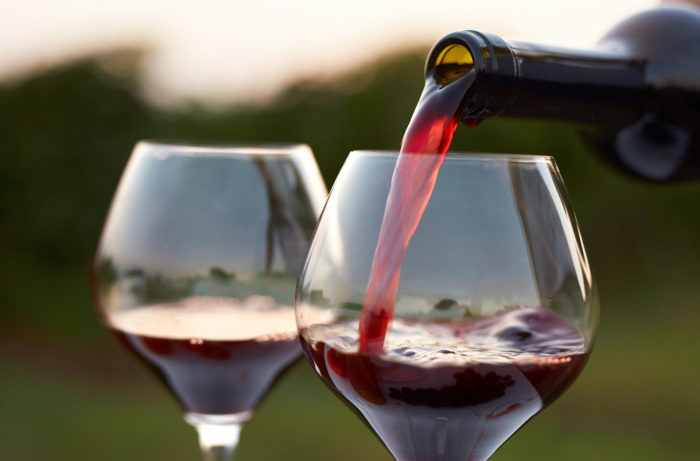
\includegraphics{vinho-verde.jpg}
\caption{Vinho Verde wine quality}
\end{figure}

\begin{Shaded}
\begin{Highlighting}[]
\CommentTok{# CHOOSE FILE TO ANALYSE: Please use 'Red_Wine.csv'}
\NormalTok{redwine <-}\StringTok{ }\KeywordTok{read.csv}\NormalTok{(}\KeywordTok{file.choose}\NormalTok{(), }\DataTypeTok{header =} \OtherTok{TRUE}\NormalTok{, }\DataTypeTok{sep =} \StringTok{","}\NormalTok{)}
\end{Highlighting}
\end{Shaded}

\clearpage

\hypertarget{the-business-problem}{%
\section{1. The Business Problem}\label{the-business-problem}}

Our winery in the Northwest of Portugal produces Vinho Verde wine. More
recently we have seen the quality of our red wine decline, each year
losing spots at the internationally acclaimed ``Best of Vinho Verde
awards''.

\begin{figure}
\centering
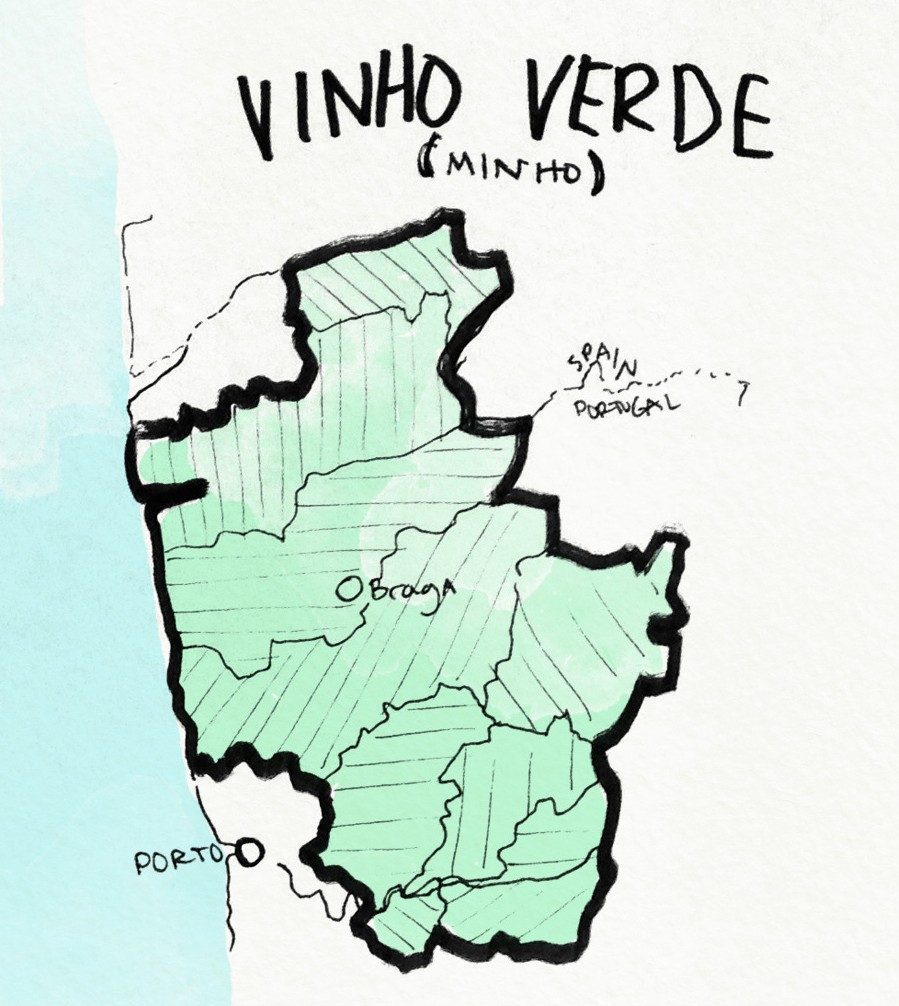
\includegraphics{Portugal_vinho_verde.jpg}
\caption{Vinho Verde production in Portugal}
\end{figure}

We are wondering if there is anything we could do to improve the quality
and rating of the wine by impacting the production process and influence
some physiochemical characteristics of the wine. Our rational is that
the grapes are the same as our competitors so there is certainly room
for improvement. We have a limited budget to work on the improvement of
our wine and would like to understand which components matter most and
how to invest to improve them.

We gathered data from 1599 red Vinho Verde wines with their measurable
characteristics:

\begin{enumerate}
\def\labelenumi{\arabic{enumi}.}
\tightlist
\item
  Fixed acidity (tartaric acid - g / dm\textsuperscript{3}): most acids
  involved with wine or fixed or nonvolatile (do not evaporate readily).
\item
  Volatile acidity (acetic acid - g / dm\textsuperscript{3}): the amount
  of acetic acid in wine, which at too high of levels can lead to an
  unpleasant, vinegar taste.
\item
  Citric acid (g / dm\textsuperscript{3}): found in small quantities,
  citric acid can add `freshness' and flavor to wines
\item
  Residual sugar (g / dm\textsuperscript{3}): the amount of sugar
  remaining after fermentation stops, it's rare to find wines with less
  than 1 gram/liter and wines with greater than 45 grams/liter are
  considered sweet.
\item
  Chlorides (sodium chloride - g / dm\textsuperscript{3}): the amount of
  salt in the wine.
\item
  Free sulfur dioxide (mg / dm\textsuperscript{3}): the free form of
  SO\textsubscript{2} exists in equilibrium between molecular
  SO\textsubscript{2} (as a dissolved gas) and bisulfite ion; it
  prevents microbial growth and the oxidation of wine.
\item
  Total sulfur dioxide (mg / dm\textsuperscript{3}): amount of free and
  bound forms of S0\textsubscript{2}; in low concentrations,
  SO\textsubscript{2} is mostly undetectable in wine, but at free SO2
  concentrations over 50 ppm, SO\textsubscript{2} becomes evident in the
  nose and taste of wine
\item
  Density (g / cm\textsuperscript{3}): the density of water is close to
  that of water depending on the percent alcohol and sugar content
\item
  pH: describes how acidic or basic a wine is on a scale from 0 (very
  acidic) to 14 (very basic); most wines are between 3-4 on the pH scale
\item
  Sulphates (potassium sulphate - g / dm\textsuperscript{3}): a wine
  additive which can contribute to sulfur dioxide gas
  (S0\textsubscript{2}) levels, wich acts as an antimicrobial and
  antioxidant
\item
  Alcohol (\% by volume): the percent alcohol content of the wine
\end{enumerate}

The expert quality rating has been calculated as the median of 3
evaluations made by experts purely based on their sensorial experience
of tasting the wines.

\clearpage

\hypertarget{the-summary-statistics-table-for-our-dataset}{%
\section{2. The Summary Statistics Table for Our
Dataset}\label{the-summary-statistics-table-for-our-dataset}}

The basic structure of the data is as follows:

\begin{verbatim}
## 'data.frame':    1599 obs. of  12 variables:
##  $ fixed.acidity       : num  7.4 7.8 7.8 11.2 7.4 7.4 7.9 7.3 7.8 7.5 ...
##  $ volatile.acidity    : num  0.7 0.88 0.76 0.28 0.7 0.66 0.6 0.65 0.58 0.5 ...
##  $ citric.acid         : num  0 0 0.04 0.56 0 0 0.06 0 0.02 0.36 ...
##  $ residual.sugar      : num  1.9 2.6 2.3 1.9 1.9 1.8 1.6 1.2 2 6.1 ...
##  $ chlorides           : num  0.076 0.098 0.092 0.075 0.076 0.075 0.069 0.065 0.073 0.071 ...
##  $ free.sulfur.dioxide : num  11 25 15 17 11 13 15 15 9 17 ...
##  $ total.sulfur.dioxide: num  34 67 54 60 34 40 59 21 18 102 ...
##  $ density             : num  0.998 0.997 0.997 0.998 0.998 ...
##  $ pH                  : num  3.51 3.2 3.26 3.16 3.51 3.51 3.3 3.39 3.36 3.35 ...
##  $ sulphates           : num  0.56 0.68 0.65 0.58 0.56 0.56 0.46 0.47 0.57 0.8 ...
##  $ alcohol             : num  9.4 9.8 9.8 9.8 9.4 9.4 9.4 10 9.5 10.5 ...
##  $ quality             : int  5 5 5 6 5 5 5 7 7 5 ...
\end{verbatim}

A summary of the data can be found below:

\begin{verbatim}
##  fixed.acidity   volatile.acidity  citric.acid    residual.sugar  
##  Min.   : 4.60   Min.   :0.1200   Min.   :0.000   Min.   : 0.900  
##  1st Qu.: 7.10   1st Qu.:0.3900   1st Qu.:0.090   1st Qu.: 1.900  
##  Median : 7.90   Median :0.5200   Median :0.260   Median : 2.200  
##  Mean   : 8.32   Mean   :0.5278   Mean   :0.271   Mean   : 2.539  
##  3rd Qu.: 9.20   3rd Qu.:0.6400   3rd Qu.:0.420   3rd Qu.: 2.600  
##  Max.   :15.90   Max.   :1.5800   Max.   :1.000   Max.   :15.500  
##    chlorides       free.sulfur.dioxide total.sulfur.dioxide
##  Min.   :0.01200   Min.   : 1.00       Min.   :  6.00      
##  1st Qu.:0.07000   1st Qu.: 7.00       1st Qu.: 22.00      
##  Median :0.07900   Median :14.00       Median : 38.00      
##  Mean   :0.08747   Mean   :15.87       Mean   : 46.47      
##  3rd Qu.:0.09000   3rd Qu.:21.00       3rd Qu.: 62.00      
##  Max.   :0.61100   Max.   :72.00       Max.   :289.00      
##     density             pH          sulphates         alcohol     
##  Min.   :0.9901   Min.   :2.740   Min.   :0.3300   Min.   : 8.40  
##  1st Qu.:0.9956   1st Qu.:3.210   1st Qu.:0.5500   1st Qu.: 9.50  
##  Median :0.9968   Median :3.310   Median :0.6200   Median :10.20  
##  Mean   :0.9967   Mean   :3.311   Mean   :0.6581   Mean   :10.42  
##  3rd Qu.:0.9978   3rd Qu.:3.400   3rd Qu.:0.7300   3rd Qu.:11.10  
##  Max.   :1.0037   Max.   :4.010   Max.   :2.0000   Max.   :14.90  
##     quality     
##  Min.   :3.000  
##  1st Qu.:5.000  
##  Median :6.000  
##  Mean   :5.636  
##  3rd Qu.:6.000  
##  Max.   :8.000
\end{verbatim}

The correlation of the data is shown in the graph below

\includegraphics{DSB_19D_G03_FinalProjectProposal_3_files/figure-latex/unnamed-chunk-3-1.pdf}

\clearpage

\hypertarget{the-business-solution-process}{%
\section{3. The Business Solution
Process}\label{the-business-solution-process}}

We are thus exploring whether there is a link between purely
physiochemical characteristics and perceived quality of the wines in
order to tailor our production process to consumer preferences in order
to achieve consistent quality of our wines. To conduct this analysis, we
plan to execute the following steps:

\begin{enumerate}
\def\labelenumi{\arabic{enumi}.}
\tightlist
\item
  Descriptive statistics of the data (preview summary above)
\item
  Select the variables that will be relevant for the model
\item
  Review the data for outliers, clean if needed, and create additional
  factors or variables as we see fit
\item
  Split the data into a training and a test data set
\item
  Conduct regression analysis on the training data set
\item
  Explore value of further analysis (e.g., factor analysis and
  segmentation)
\item
  Develop different models to predict the best wine
\item
  Evaluate our different models using the test data set
\item
  Select the model with the less errors in the predictions
\end{enumerate}

Once we have the best model, we will be able to know the characteristics
that make a great wine. We will be able to adapt our production process
in order to produce a wine that will win awards, use our investment
resources in the most effective way and that will appeal to the
customers.

\clearpage


\end{document}
